Haizea is an open-source VM-based lease management architecture. Let's break that down, shall we?

\begin{description}
\item[Haizea is a resource manager] (or, depending on who you ask, a "resource scheduler"): Haizea is a software component that can manage a set of computers (typically a cluster), allowing users to request exclusive use of those resources described in a variety of terms, such as "I need 10 nodes, each with 1 GB of memory, right now" or "I need 4 nodes, each with 2 CPUs and 2GB of memory, from 2pm to 4pm tomorrow".
\item[Haizea uses leases] The fundamental resource provisioning abstraction in Haizea is the lease. Intuitively, a lease is some form of contract where one party agrees to provide a set of resources (an apartment, a car, etc.) to another party. When a user wants to request computational resources from Haizea, it does so in the form of a lease. When applied to computational resources, the lease abstraction is a powerful and general construct with a lot of nuances. See below for a more detailed definition of leases or read about the types of leases supported by Haizea.
\item[Haizea is VM-based] We hold that the best way of implementing resource leases is using virtual machines (VMs). Therefore, Haizea's scheduling algorithms are geared towards managing virtual machines, factoring in all the extra operations (and overhead) involved in managing VMs. The Globus Virtual Workspaces group, where Haizea was originally developed, has an extensive list of publications that argue how using virtual machines for resource leasing is A Good Thing (and also Not A Trivial Thing).
\item[Haizea is open source] Haizea is published under the Apache License 2.0, a BSD-like OSI-compatible license.
\end{description}

\section{What can you do with Haizea?}

\begin{center}
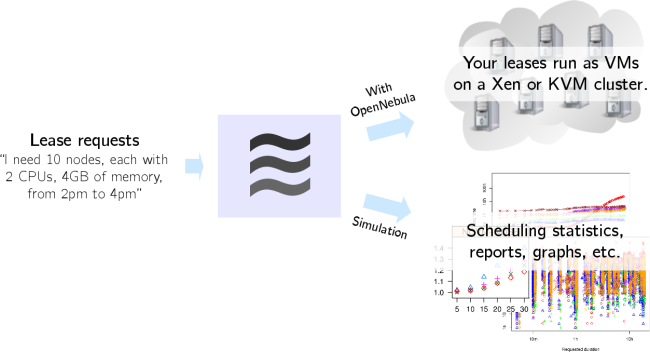
\includegraphics{images/what_haizea_does.png}
\end{center}


You can use Haizea one of two ways. Haizea can be used as a standalone component or as a scheduling backend for a virtual infrastructure manager, such as OpenNebula. So, if you're...

\begin{description}
\item[Using Haizea with OpenNebula] Haizea can be used as a drop-in replacement for OpenNebula's scheduling daemon. OpenNebula is a virtual infrastructure manager that enables the dynamic deployment and re-allocation of virtual machines on a pool of physical resources. OpenNebula and Haizea complement each other, since OpenNebula provides all the enactment muscle (OpenNebula can manage Xen and KVM virtual machines on a cluster, with VMWare support to follow shortly) while Haizea provides all the scheduling brains. The document "Using OpenNebula and Haizea to manage VMs on a cluster" provides more details on how to use OpenNebula 1.0 and Haizea together.
\item[Using Haizea on its own] In this case, you actually can't do all that much :-) Haizea is, primarily, a VM resource management component that can take lease requests and make scheduling decisions, but doesn't actually know anything about how to enact those decisions. For example, Haizea may determine at what times a set of VMs representing a lease must start and stop, but it doesn't actually know how to instruct a virtual machine manager to do these actions. Haizea can, however, simulate those enactment actions so, on its own, Haizea might be useful if you're doing scheduling research involving leases or VMs (in fact, the Haizea simulator has been used in a couple of papers).
\end{description}

You can find a couple (more specific) details about what you can do with Haizea in our list of features.

\begin{description}
 \item[Simulation mode, simulated time:] In this mode, Haizea works with a simulated set of hardware resources (which we'll be able to specify in a configuration file). When a lease is scheduled, all enactment commands (``start VM'', ``stop VM'', etc.) for that lease are simulated. Additionally, when time is simulated, Haizea will just ``fast forward'' through all the lease requests it receives. For example, suppose you've requested a lease that requires 30
 \item[Simulation mode, real time:]  The ``real time'' mode simply means that time will pass
 \item[OpenNebula mode:] 
\end{description}


\section{Leasing as a fundamental abstraction}

% Include very short spiel

\section{Features}

Foobar

\section{Haizea is extensible}

The Haizea architecture has been designed so it can be used as a scheduling component that can be plugged into other systems by implementing a set of extra modules in Haizea using a well-defined API (i.e., without having to modify the core of Haizea). Right now, Haizea depends on OpenNebula to perform enactment actions on real systems (and, in turn, OpenNebula can use Haizea as its scheduling backend), but Haizea could be made to work with other systems with relative ease. See the Haizea architecture page for more details.

\section{Haizea is still a technology preview}

Haizea started out as research software (and it is still largely meant for research purposes). Although Haizea works and we're getting to the point where it can be used in production systems, it is still a technology preview, so please use it with caution. In particular, although we've produced some documentation and polished up the code, there is still a fair amount of documentation that has to be produced. If you have any trouble using Haizea, or understanding any part of the source code, please don't hesitate to ask for help.